\newcommand{\Subject}{\LARGE \bf Navigation without localisation:\\--\\ reliable teach and repeat based on the convergence theorem}
\newcommand{\Meeting}{IROS'18 Presentation on exposure and detector setting experiments' outcomes}
\newcommand{\Authors}{Tom{\' a}{\v s} Krajn{\'i}k, Filip Majer, Lucie Halodov{\' a}, Tom{\' a}{\v s} Vintr}
\newcommand{\Author}{Tom Krajnik}
\newcommand{\Date}{October 2018}
%\usetheme{warsaw}

\newcommand{\video}[2]{\href{run:#1}{\includegraphics[width=0.99\textwidth]{#2}}}
%\newcommand{\link}[2]{\href{run:#1}{\includegraphics[width=0.99\textwidth]{#2}}}
\newcommand{\bib}[3]{\begin{thebibliography}{#1}\bibitem[#1]{#1}{#2}.\newblock{\em #3}\end{thebibliography}}

\newcommand{\Lincoln}{Artificial Intelligence Centre, Czech Technical University, Czechia}
\newcommand{\Institute}{\Lincoln\\}

\newcommand{\HeadLineLeft}{Krajn{\' i}k et al.}
\newcommand{\HeadLineCenter}{Navigation without localisation: reliable teach and repeat based on the convergence theorem}
\newcommand{\HeadLineRight}{Madrid, IROS 2018}
\newcommand{\FootLineCenter}{Navigation without localisation: reliable teach and repeat based on the convergence theorem}
\newcommand{\FootLineLeft}{\insertshortauthor}

% File name: head.tex
% Date:      2008/09/28 20:40
% Author:    Jan Faigl

\newread\testin
\def\softinput #1 {\let\next=\relax \openin\testin=#1
\ifeof\testin \message{Info: the file #1 does not exist}%
\else \closein\testin \def\next{\input #1 }\fi
\next}

\softinput{makeconfig}

\ifx\print\undefined
\documentclass[mathserif]{beamer}
% File name: head-beamer.tex
% Date:      2008/09/28 20:40
% Author:    Jan Faigl

%\usepackage[latin2]{inputenc}
%\usepackage{times}
\usepackage[T1]{fontenc}
\usepackage{helvet}
\usepackage{graphicx}
\usepackage{multimedia}
\usepackage{hyperref}
\usepackage{amsmath}
\usepackage{textcomp}

\usepackage{listings}
\usepackage{ragged2e}

\lstset{extendedchars=true}
\lstset{inputencoding=latin2}
\lstset{breaklines=true,basicstyle=\tiny,language=sh}
\lstset{language=java}
\lstset{columns=fullflexible}
\definecolor{background_color}{gray}{0.9}
\definecolor{comment_color}{rgb}{0.0, 0.5, 0.0}
\definecolor{keyword_color}{rgb}{0.0, 0.0, 1.0}
\definecolor{string_color}{rgb}{0.8, 0.0, 0.0}

\lstset{keywordstyle=\color{keyword_color}\bfseries}
\lstset{commentstyle=\color{comment_color}}
\lstset{stringstyle=\color{string_color}}
\lstset{basicstyle=\ttfamily}
\lstset{showstringspaces=false}
\lstset{keepspaces=true}
\lstset{tabsize=2}
\lstset{breaklines=true}

\institute{\Institute}

\date{\Date}
\author[\Author]{\Authors}
\newcommand{\disable}[1]{}

\colorlet{redshaded}{red!25!bg}
\colorlet{shaded}{black!25!bg}
\colorlet{shadedshaded}{black!10!bg}
\colorlet{blackshaded}{black!40!bg}

\colorlet{darkred}{red!80!black}
\colorlet{darkblue}{blue!80!black}
\colorlet{darkgreen}{green!80!black}

\newcommand{\myurl}[1]{{\color{blue}\url{#1}}}

\DeclareMathOperator{\argmax}{argmax}

\pgfdeclareimage[height=0.4cm]{GL}{fig/gl-logo}
\pgfdeclareimage[height=1.0cm]{logoGL}{fig/logoGL}
%\logo{\pgfuseimage{GL}}
\logo{\pgfuseimage{logoGL}}

\usetheme{Singapore}

\setbeamercovered{transparent}
\setbeamertemplate{navigation symbols}{ }

\defbeamertemplate*{part page}{}[1][]{
\begin{centering}
   {\usebeamerfont{part name}\usebeamercolor[fg]{part name}Part~\insertromanpartnumber}
   \vskip1em\par
   \begin{beamercolorbox}[sep=8pt,center,#1]{part title}
      \usebeamerfont{part title}\insertpart\par
   \end{beamercolorbox}
\end{centering}
}        

\setbeamerfont{code}{size={\fontsize{11pt}{6pt}}}
\setbeamerfont{codeSmall}{size={\fontsize{10pt}{6pt}}}
\setbeamerfont{codeSmaller}{size={\fontsize{9pt}{6pt}}}
\setbeamerfont{small}{size={\fontsize{8pt}{6pt}}}
\AtBeginPart{\frame{\partpage}}


\setbeamercolor{alerted text}{fg=red!80!black}

%-----------------------------------------------------------------------------
% Header line
%-----------------------------------------------------------------------------

\defbeamertemplate*{headline}{}
{%
\begin{beamercolorbox}[colsep=1.5pt]{upper separation line head}
\end{beamercolorbox}
\hbox{%
\begin{beamercolorbox}[wd=0.15\paperwidth,ht=2.25ex,dp=1ex,left]{section in head/foot}%
   \usebeamerfont{title in head/foot}\hspace*{2ex}\HeadLineLeft\hspace*{2ex}
\end{beamercolorbox}%
\begin{beamercolorbox}[wd=0.7\paperwidth,ht=2.25ex,dp=1ex,center]{subsection in head/foot}%
  \usebeamerfont{subsection in head/foot}\hspace*{2ex}\HeadLineCenter
\end{beamercolorbox}%
\begin{beamercolorbox}[wd=0.15\paperwidth,ht=2.25ex,dp=1ex,left]{section in head/foot}%
   \usebeamerfont{section in head/foot}\hspace*{1ex}\HeadLineRight
\end{beamercolorbox}%
}
%\begin{beamercolorbox}{section in head/foot}
%   \vskip2pt\insertsectionnavigationhorizontal{\paperwidth}{}{}\vskip2pt
% \end{beamercolorbox}%

\begin{beamercolorbox}[colsep=1.5pt]{lower separation line head}
\end{beamercolorbox}
}
\addtoheadtemplate{\pgfuseshading{beamer@headfade}\vskip-1.25cm}{}

%-----------------------------------------------------------------------------
% footline
%-----------------------------------------------------------------------------
\defbeamertemplate*{footline}{}{
\leavevmode%
\hbox{%
\begin{beamercolorbox}[wd=.22\paperwidth,ht=2.25ex,dp=1ex,left]{author in head/foot}%
   \usebeamerfont{author in head/foot}\hspace*{2ex}\FootLineLeft\hspace*{2ex}
\end{beamercolorbox}%
\begin{beamercolorbox}[wd=.68\paperwidth,ht=2.25ex,dp=1ex,center]{institute in head/foot}%
   \usebeamerfont{title in head/foot}\FootLineCenter
\end{beamercolorbox}%
\begin{beamercolorbox}[wd=0.1\paperwidth,ht=2.25ex,dp=1ex,right]{date in head/foot}%
   \insertframenumber{} / \inserttotalframenumber\hspace*{1ex}
\end{beamercolorbox}}%
\vskip0pt%
}

\else
\documentclass[trans]{beamer}
% File name: head-print.tex
% Date:      2008/09/28 20:40
% Author:    Jan Faigl

\usepackage[latin2]{inputenc}
\usepackage{times}
\usepackage[T1]{fontenc}
\usepackage{helvet}
\usepackage{graphicx}
\usepackage{multimedia}
\usepackage{hyperref}
\usepackage{amsmath}
\usepackage{textcomp}

\usepackage{listings}
\usepackage{ragged2e}

\lstset{extendedchars=true}
\lstset{inputencoding=latin2}
\lstset{breaklines=true,basicstyle=\tiny,language=sh}
\lstset{language=java}
\lstset{columns=fullflexible}
\definecolor{background_color}{gray}{0.9}
\definecolor{comment_color}{rgb}{0.0, 0.5, 0.0}
\definecolor{keyword_color}{rgb}{0.0, 0.0, 1.0}
\definecolor{string_color}{rgb}{0.8, 0.0, 0.0}

\lstset{keywordstyle=\color{keyword_color}\bfseries}
\lstset{commentstyle=\color{comment_color}}
\lstset{stringstyle=\color{string_color}}
\lstset{basicstyle=\ttfamily}
\lstset{showstringspaces=false}
\lstset{keepspaces=true}
\lstset{tabsize=2}
\lstset{breaklines=true}

\institute{\Institute}

\date{\Date}
\author[\Author]{\Subject}
\newcommand{\disable}[1]{}

\colorlet{redshaded}{red!25!bg}
\colorlet{shaded}{black!25!bg}
\colorlet{shadedshaded}{black!10!bg}
\colorlet{blackshaded}{black!40!bg}

\colorlet{darkred}{red!80!black}
\colorlet{darkblue}{blue!80!black}
\colorlet{darkgreen}{green!80!black}

\newcommand{\myurl}[1]{{\color{blue}\url{#1}}}

\DeclareMathOperator{\argmax}{argmax}

\pgfdeclareimage[height=0.4cm]{GL}{fig/gl-logo}
\pgfdeclareimage[height=0.4cm]{logoGL}{fig/logoGL}
\logo{\pgfuseimage{GL}}
%\logo{\pgfuseimage{logoGL}}

\usetheme{default}

\setbeamercovered{transparent}
\setbeamertemplate{navigation symbols}{ }

\defbeamertemplate*{part page}{}[1][]{
\begin{centering}
   {\usebeamerfont{part name}\usebeamercolor[fg]{part name}��st~\insertromanpartnumber}
   \vskip1em\par
   \begin{beamercolorbox}[sep=8pt,center,#1]{part title}
      \usebeamerfont{part title}\insertpart\par
   \end{beamercolorbox}
\end{centering}
}        

\setbeamerfont{code}{size={\fontsize{11pt}{6pt}}}
\setbeamerfont{codeSmall}{size={\fontsize{10pt}{6pt}}}
\setbeamerfont{codeSmaller}{size={\fontsize{9pt}{6pt}}}
\setbeamerfont{small}{size={\fontsize{8pt}{6pt}}}
\AtBeginPart{\frame{\partpage}}


\setbeamercolor{alerted text}{fg=red!80!black}


%-----------------------------------------------------------------------------
% footline
%-----------------------------------------------------------------------------
\defbeamertemplate*{footlineX}{}{
\leavevmode%
\hbox{%
\begin{beamercolorbox}[wd=.34\paperwidth,ht=2.25ex,dp=1ex,left]{author in head/foot}%
   \usebeamerfont{author in head/foot}\hspace*{2ex}\FootLineLeft\hspace*{2ex}
\end{beamercolorbox}%
\begin{beamercolorbox}[wd=.51\paperwidth,ht=2.25ex,dp=1ex,center]{institute in head/foot}%
   \usebeamerfont{title in head/foot}\FootLineCenter
\end{beamercolorbox}%
\begin{beamercolorbox}[wd=0.14\paperwidth,ht=2.25ex,dp=1ex,right]{date in head/foot}%
   \insertframenumber{} / \inserttotalframenumber\hspace*{1ex}
\end{beamercolorbox}}%
\vskip0pt%
}

\fi



\title{{\bf \Subject}}
\usepackage{multirow}
\begin{document}
% - frame ---------------------------------------------------------------------

\frame{\titlepage}

% - frame --------------------------------------------------------------------
\begin{frame}
   \frametitle{Map-based Visual Navigation}
	\begin{columns}
	\hfill
	\column{0.45\textwidth}
	Visual navigation:
   \begin{enumerate}
	   \item  Extract image features,
	   \item  find correspondences,
	   \item  determine robot pose,
	   \item  calculate movement.
   \end{enumerate}
	\column{0.45\textwidth}
\only<2,3,4>{
	Problems:
   \begin{enumerate}
	   \item  Feature deficiency,
	   \item  environment change,
	   \item  precision, complexity,
	   \item  real-time issues.
   \end{enumerate}
}
   \end{columns}
	 \vfill
	 \only<1,2,3>{\invisible<1,2>{\hfill\includegraphics[width=0.45\textwidth]{fig/hostibejk_day}\hfill\includegraphics[width=0.45\textwidth]{fig/hostibejk_night}\hfill}}
      \vfill
\only<4>{
	To overcome the aforementioned problems, you a \textbf{realistic} model of position uncertainty. Investigating how the uncertainties robot position ($x,y$) and heading ($\varphi$) affect each other, several authors have concluded that error of the robot heading ($\varphi$) estimation has a significantly more prominent impact thab $(x,y)$ error.
      \vfill
}
\end{frame}

\section{Method principle}
% - frame ---------------------------------------------------------------------
\begin{frame}
   \frametitle{For navigation, heading estimation is crucial}

   During autonomous navigation
   \begin{itemize}
	\item the inaccurracy of $\varphi$ causes $x,y$ estimation errors, 
	\item but $x,y$ errors influence $\varphi$ estimation only marginally.
   \end{itemize}
   \vspace{5mm}
   Heading-only estimation
    \begin{itemize}
	\item is simpler and faster to calculate,
	\item requires only a low number of feature correspondences,
 	\item and is more robust than full ($x,y,\varphi)$ estimation.
   \end{itemize}
   \vspace{5mm}
  We show that in teach-and-repeat visual navigation,
    \begin{itemize}
	\item one can use the camera for \textbf{heading estimation only}, 
	\item and leave $x,y$ estimates to odometry. 
   \end{itemize}
\end{frame}

% - frame ---------------------------------------------------------------------
\begin{frame}
\frametitle{Position error evolution}
      \only<1>{\video{cmds/segment.sh}{fig/segment_one_start.jpg}}
      \only<2>{\video{cmds/segment.sh}{fig/segment_one_end.jpg}}
\end{frame}

% - frame ---------------------------------------------------------------------
\begin{frame}
\frametitle{Position error evolution}
   \begin{columns}
      \column{0.6\textwidth}
      \only<1>{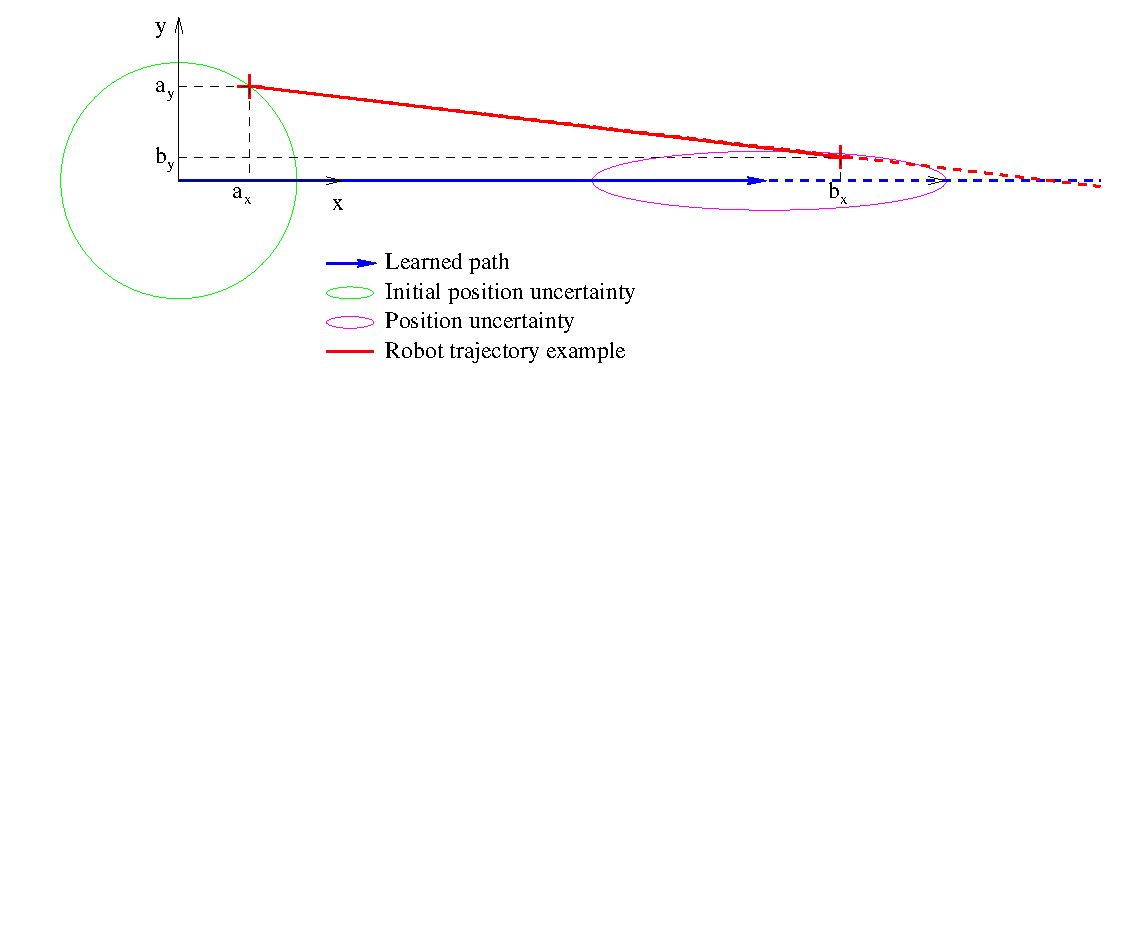
\includegraphics[width=1.2\columnwidth]{fig/converge0}}\\
      \only<2>{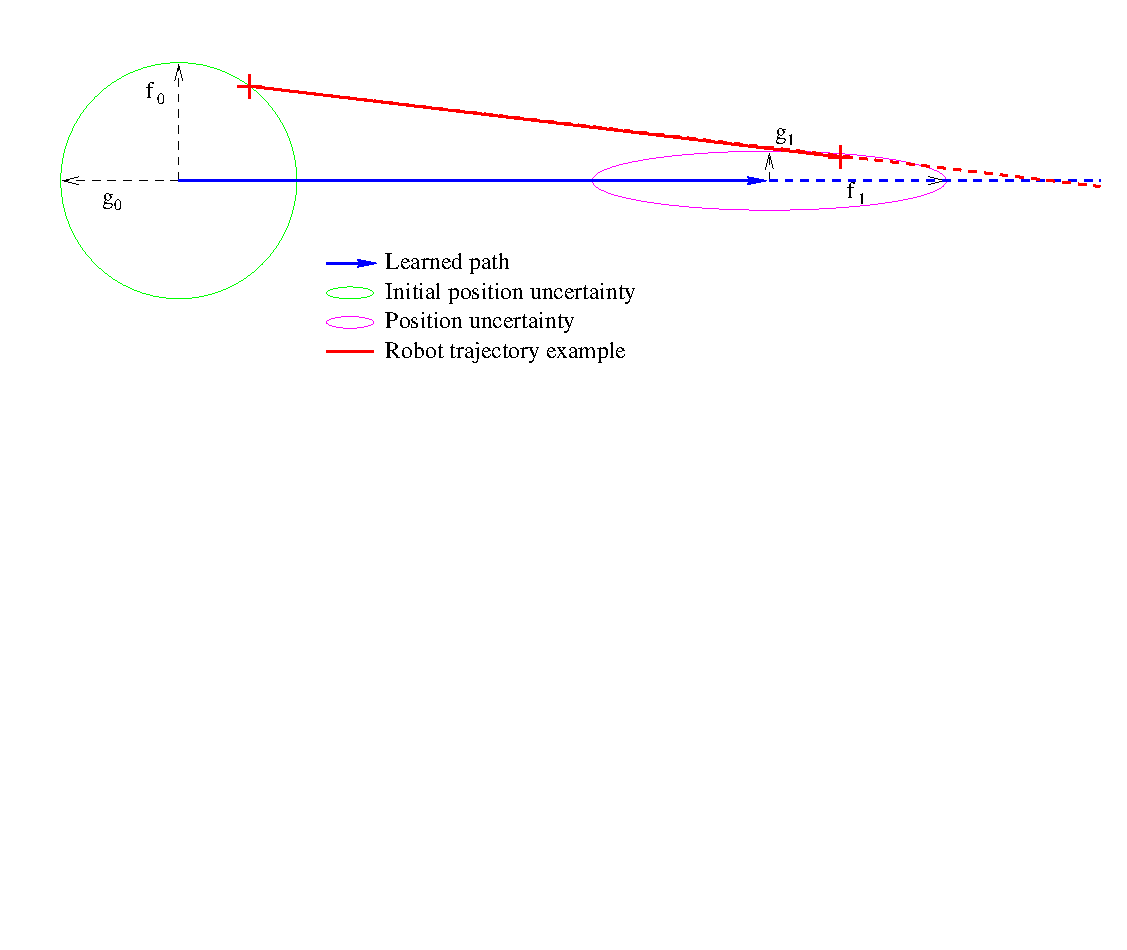
\includegraphics[width=1.2\columnwidth]{fig/converge1}}\\
      \only<3>{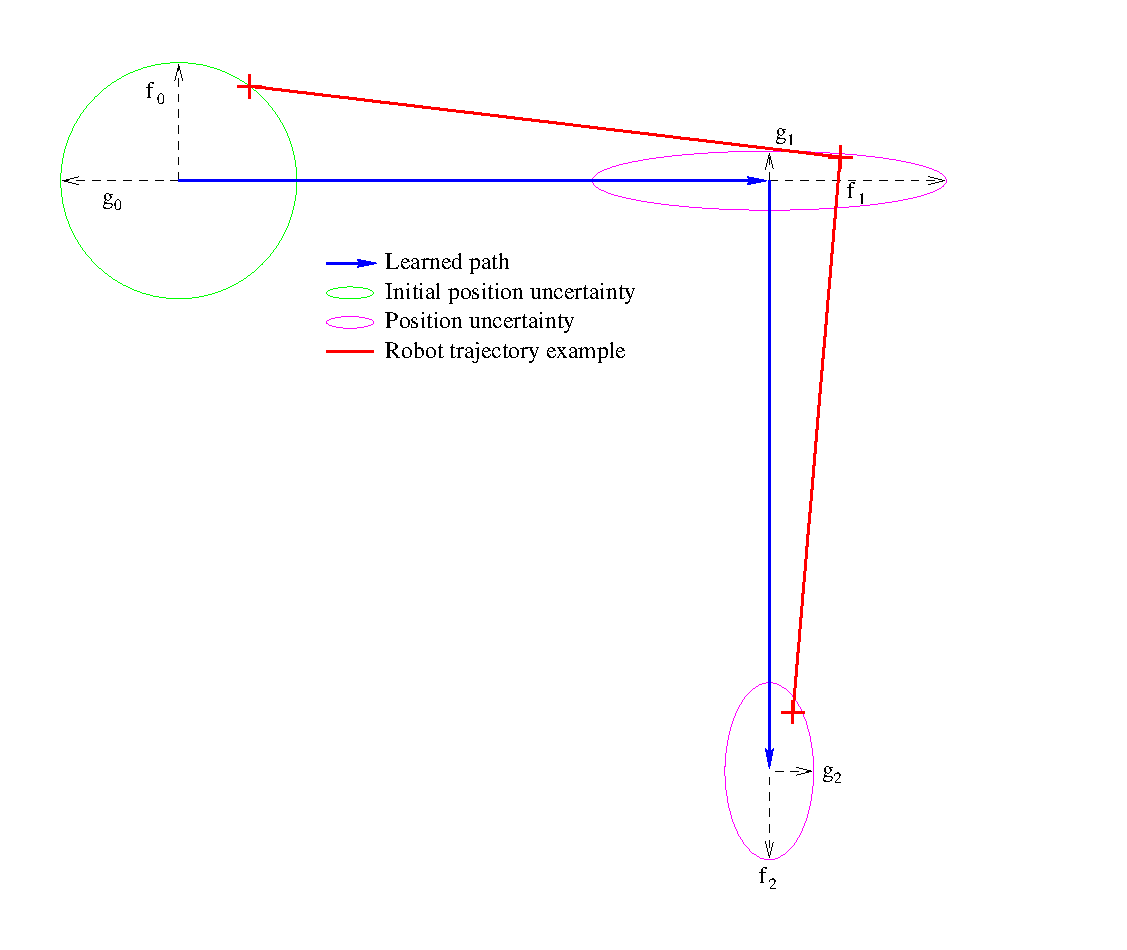
\includegraphics[width=1.2\columnwidth]{fig/converge2}}\\
      \only<4>{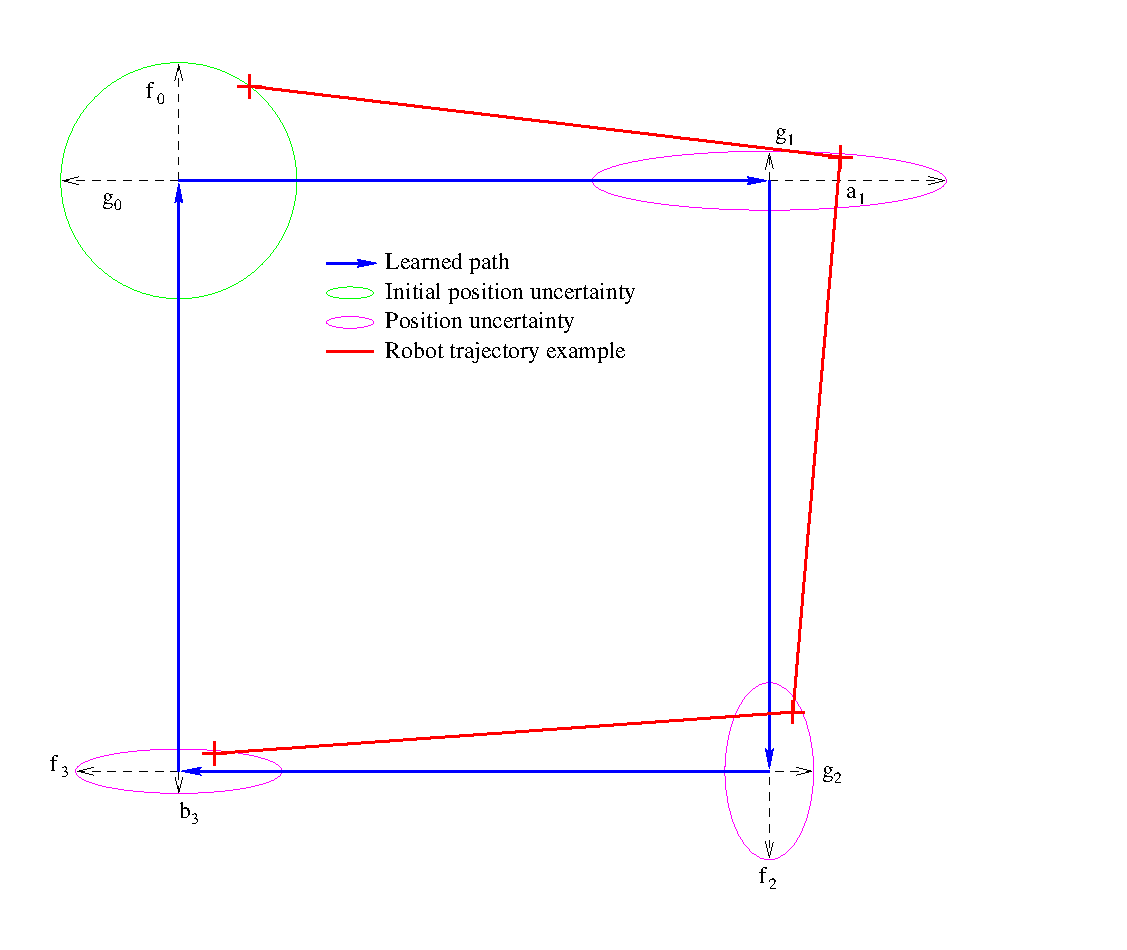
\includegraphics[width=1.2\columnwidth]{fig/converge3}}\\
      \only<5>{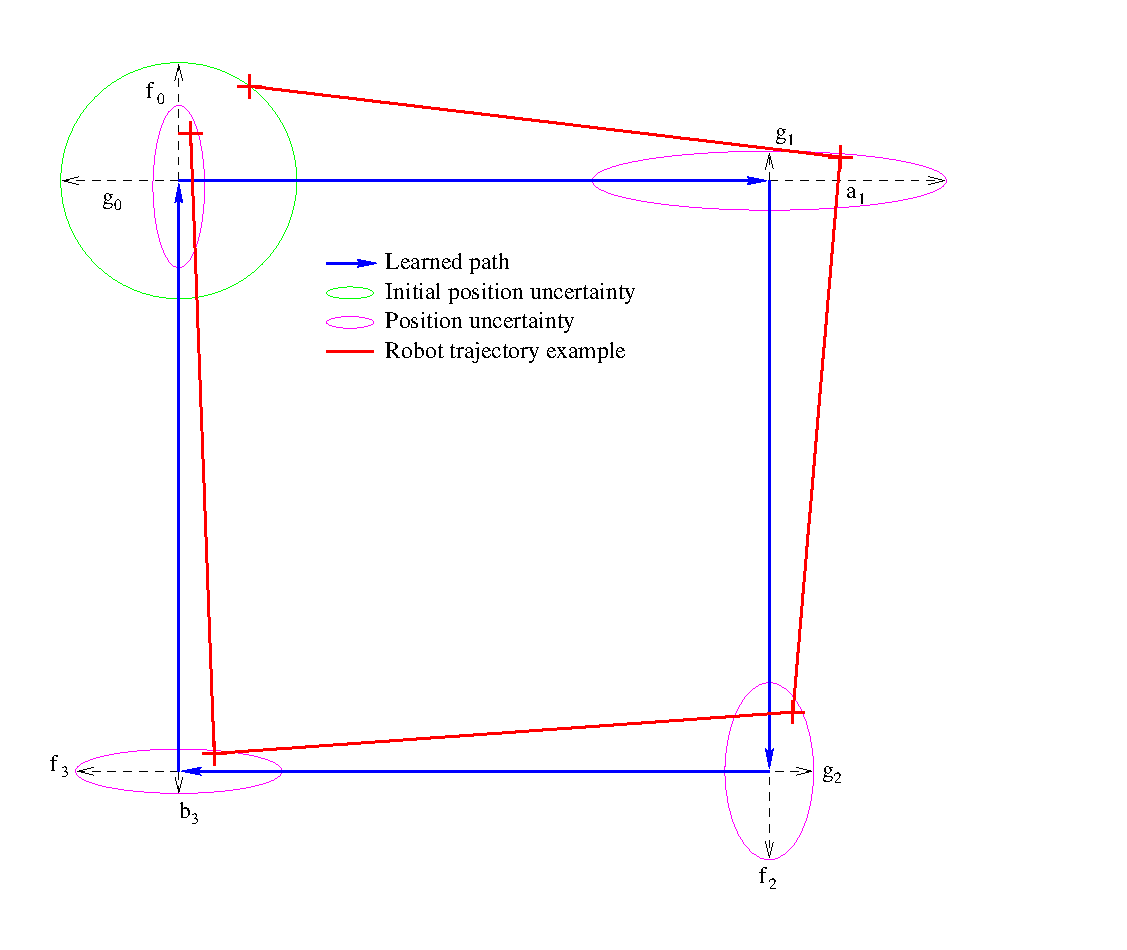
\includegraphics[width=1.2\columnwidth]{fig/converge4}}\\
      \column{0.4\textwidth}%
      Robot position coordinates 
      \begin{equation*}
	      \begin{array}{l}
		      b_x = a_x+s(1+\upsilon),\\
		      b_y = ma_y+\xi.
	      \end{array}
      \end{equation*} 
      $m$ - heading correction\\
      $\xi,\upsilon$ - errors (odo+cam)\\
      \vspace{3mm}
      \invisible<1>{
      Position error ellipse axes\\
	$f_{i+1}=g_{i}+\upsilon$, $g_{i+1}=mf_{i}+\xi$\\
      }
      \vspace{3mm}
      \invisible<1-3>{
      Convergence\\
	$f_{\infty} = (\xi+\upsilon)/(1-m)$\\ 	
	$f_{\infty}$, $g_{\infty}$ finite if $\|m\| < 1$.
      }
\end{columns}
\end{frame}

% - frame ---------------------------------------------------------------------
\begin{frame}
\frametitle{Position error evolution}
      \video{cmds/converge.sh}{fig/loop.jpg}
\end{frame}

\begin{frame}
\frametitle{Navigation at night}
      \video{cmds/night.sh}{fig/loop.jpg}
\end{frame}

\begin{frame}
	\frametitle{Experimental evaluation}
	\begin{center}
		Night  experiment.
	\end{center}
\end{frame}

% - frame ---------------------------------------------------------------------
\begin{frame}
	\frametitle{Questions}
	\begin{center}
\vfill
\vfill
	Source code available at \\
\vfill
		https://bearnav.eu\\
\vfill
		Questions? 
\vfill
\vfill
\vfill
\vfill
\vfill
	\end{center}
\end{frame}







\tiny{[1] Krajnik et al.: Simple Yet Stable Bearing Only Navigation, Journal of Field Robotics, 2010}

\section{What about odometry drift}
% - frame ---------------------------------------------------------------------
\begin{frame}
   \frametitle{For navigation, heading estimation is crucial}

   During vision-in-the-loop navigation
   \begin{itemize}
	\item the inaccurracy of $\varphi$ causes $x,y$ estimation errors, 
	\item but $x,y$ errors influence $\varphi$ estimation only marginally.
   \end{itemize}
   \vspace{5mm}
   During vision-in-the-loop navigation


   Thus, to achieve reliable navigation, one can use exteroceptive sensing to estimate $\varphi$ and leave $x,y$ estimates on odometry. 
   In other words, full 3D \textbf{localisation is not needed} and the heading correctionscan suppress odometric drift and ensure that the $x,y$ error does not diverge [1].\\ 
   Therefore we propose
   \begin{itemize}
 	\item to use the vision to estimate only the robot heading,
 	\item and leave $x,y$ position estimation just on the odometry.
   \end{itemize}
   \vspace{5mm}
   We have created a navigation system, that works in two phases
   \begin{description}
	\item[mapping] - a  map is created during a teleoperated run,
 	\item[navigation]  - the robot uses the map to navigate.
   \end{description}
   \tiny{[1] Krajnik et al.: Simple Yet Stable Bearing Only Navigation, Journal of Field Robotics, 2010}
\end{frame}


\begin{frame}
	\frametitle{Teach and repeat navigation}
   \vfill
   \begin{columns}
      \column{1.0\textwidth}
   \begin{itemize}
	\item manually guide the robot along a given path,
	\item robot remembers its velocity along the path,
	\item robot remembers image efatures that it saw,
	\item robot replays its velocities,
	\item while correcting its heading according to its visual memory.
   \end{itemize}
   \end{columns}
   \begin{center}
	 \includegraphics[width=0.85\textwidth]{fig/testpaths}
	 \vspace{-3mm}
   \end{center}
\end{frame}

\begin{frame}
\frametitle{Teach and repeat navigation}
   \begin{overlayarea}{\textwidth}{\textheight}
	 \only<1>{\includegraphics[width=1.0\textwidth]{fig/s0}}
	 \only<2>{\includegraphics[width=1.0\textwidth]{fig/s1}}
	 \only<3>{\includegraphics[width=1.0\textwidth]{fig/s2}}
	 \only<4>{\includegraphics[width=1.0\textwidth]{fig/s3}}
	 \only<5>{\includegraphics[width=1.0\textwidth]{fig/s4}}
	 \only<6>{\includegraphics[width=1.0\textwidth]{fig/s5}}
	 \only<7>{\includegraphics[width=1.0\textwidth]{fig/s6}}
	 \only<8>{\includegraphics[width=1.0\textwidth]{fig/s7}}
	 \only<9>{\includegraphics[width=1.0\textwidth]{fig/s8}}
	 \only<10>{\includegraphics[width=1.0\textwidth]{fig/s9}}
	 \only<11>{\includegraphics[width=1.0\textwidth]{fig/s10}}
   \end{overlayarea}
\end{frame}

\begin{frame}
\frametitle{Teach and repeat navigation}
	\begin{columns}
		\column{0.48\textwidth}%
		\begin{normalsize}
			Mapping phase
		\end{normalsize}
		\begin{itemize}
			\item Move forwards, remember velocities,
			\item extract and track image features,
			\item store features every 0.2~m along with robot odometry.
		\end{itemize}
		%\includegraphics[width=0.5\textwidth]{fig/method_learn.png}\\
		\column{0.52\textwidth}%
		\begin{normalsize}
			Autonomous navigation	
		\end{normalsize}
		\begin{itemize}
			\item Replay the mapped velocities,
			\item extract image features, 
			\item match them to the mapped ones,
			\item determine horizontal displacement,
			\item use to steer the robot.
		\end{itemize}
		%\includegraphics[width=0.5\textwidth]{fig/method_traverse.png}\\
	\end{columns}
\end{frame}

\begin{frame}
\frametitle{Teach and repeat navigation}
	Video navigation 1  
\end{frame}

\begin{frame}
\frametitle{Teach and repeat navigation}
	Video segment 2  
\end{frame}


\end{document}
